\documentclass[11pt,a4paper]{article}
\usepackage[T1]{fontenc}
\usepackage[utf8]{inputenc}
\usepackage{mathptmx}
\usepackage[scaled=0.92]{helvet}
\usepackage{courier}
\usepackage[margin=2.4cm]{geometry}
\usepackage{microtype}
\usepackage{amsmath}
\usepackage{booktabs}
\usepackage{tabularx}
\usepackage{xcolor}
\usepackage{tikz}
\usetikzlibrary{arrows.meta,positioning}
\usepackage{enumitem}
\usepackage[hidelinks]{hyperref}
\setlist{itemsep=2pt,topsep=4pt}
\setlength{\emergencystretch}{3em}

\title{\textbf{CiviCite}: A Verified, Citation-First Retrieval-Augmented\\ Assistant for Swedish Public Services}
\author{Varshith\\ \small Blekinge Institute of Technology (BTH), Sweden}
\date{October 2026}

\begin{document}
\maketitle

\begin{abstract}
People navigating Swedish public services, especially newcomers, need answers that are correct, current and
traceable to an official source. General-purpose chatbots fail in exactly the ways that matter here: they
invent deadlines, amounts and rules. CiviCite is a retrieval-augmented assistant built around three guarantees.
Every factual sentence must cite a retrieved source. A sentence-level verifier checks term overlap and
\emph{number consistency} against the cited text. The system abstains when the evidence is weak.
Date arithmetic, a frequent source of errors, is delegated to a deterministic tool that implements the
Swedish calendar rules. Personal identity numbers and other personal data are redacted before any text
reaches a model or a log, and retrieved passages that attempt prompt injection are discarded. On a
34-question development set, the LLM-free extractive baseline reaches 1.00 retrieval recall@5,
0.846 answer accuracy, 0.857 abstention F1 and 1.00 faithfulness, with sub-millisecond latency. An
evaluation harness gates these numbers in continuous integration and runs the same suite against any
OpenAI-compatible model.
\end{abstract}

\section{Introduction}
Retrieval-augmented generation (RAG)~\cite{lewis} grounds language models in external documents, but
grounding alone does not guarantee faithfulness: models still mix retrieved facts with parametric memory,
cite the wrong passage, or answer questions the documents do not cover~\cite{alce,ragas}. In public-service
guidance the cost of such errors is concrete: a wrong deadline for reporting a move (\emph{flyttanmälan})
or for applying for temporary parental benefit (VAB) can mean fees or lost benefits.

CiviCite treats \emph{verifiability} as the primary design goal rather than fluency:
\begin{itemize}
  \item \textbf{Citation-first answers}: every claim carries a source number, and the UI shows the cited text.
  \item \textbf{Post-hoc verification}: each sentence is checked against its cited source, and unsupported
        sentences are flagged (or, in strict mode, the answer is replaced by an abstention).
  \item \textbf{Calibrated abstention}: an evidence score decides when to answer at all.
  \item \textbf{Deterministic tools} for date arithmetic, following the Swedish rule that statutory deadlines
        falling on a Saturday, Sunday, public holiday, Midsummer Eve, Christmas Eve or New Year's Eve move to
        the next working day~\cite{lag1930}.
  \item \textbf{Privacy and robustness}: Luhn-validated redaction of \emph{personnummer} and
        \emph{samordningsnummer}, e-mail, phone, IBAN and card numbers, and an indirect-prompt-injection
        filter for retrieved text~\cite{greshake}.
\end{itemize}

\section{System design}
\begin{figure}[h]
\centering
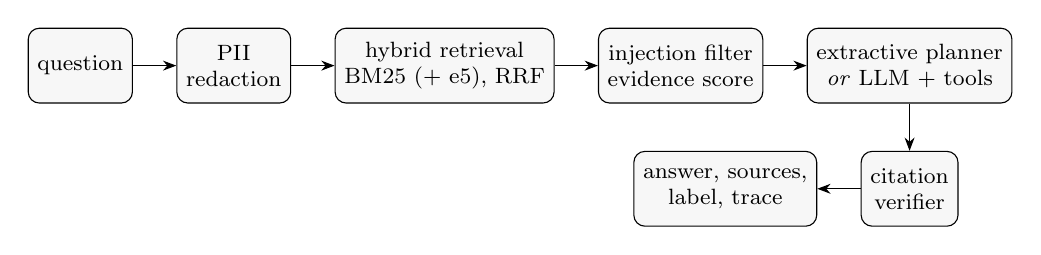
\begin{tikzpicture}[node distance=0.45cm and 0.55cm, box/.style={draw,rounded corners,align=center,
  font=\footnotesize,minimum height=0.95cm,fill=black!3}, >={Stealth}]
\node[box] (q) {question};
\node[box,right=of q] (p) {PII\\redaction};
\node[box,right=of p] (r) {hybrid retrieval\\BM25 (+ e5), RRF};
\node[box,right=of r] (g) {injection filter\\evidence score};
\node[box,right=of g] (a) {extractive planner\\ \emph{or} LLM + tools};
\node[box,below=0.6cm of a] (v) {citation\\verifier};
\node[box,left=of v] (o) {answer, sources,\\label, trace};
\draw[->] (q)--(p); \draw[->] (p)--(r); \draw[->] (r)--(g); \draw[->] (g)--(a); \draw[->] (a)--(v); \draw[->] (v)--(o);
\end{tikzpicture}
\caption{CiviCite pipeline.}
\end{figure}

\paragraph{Ingestion.} Markdown, HTML (navigation, scripts and footers removed, headings preserved) and PDF
documents are split into heading-aware chunks that never span two sections. Each chunk keeps its title,
section, agency and URL. A polite crawler (robots.txt, rate limiting, prefix-restricted, de-duplicated by
content hash) converts agency web pages into this format.

\paragraph{Retrieval.} BM25~\cite{bm25} over stop-word-filtered, lightly stemmed English/Swedish terms
is fused with optional multilingual E5 embeddings~\cite{e5} by reciprocal rank fusion~\cite{rrf}. A small
Swedish$\to$English glossary expands queries when the corpus language differs from the question language.

\paragraph{Evidence score and abstention.} For query terms $T$ (each with its glossary alternatives) and a
chunk $c$, the IDF-weighted coverage is
\[
  \mathrm{cov}(c) = \frac{\sum_{t \in T} w_t \cdot \mathbf{1}[t \in c]}{\sum_{t \in T} w_t}, \qquad
  w_t = \begin{cases} \mathrm{idf}(t) & t \text{ in collection} \\ \max \mathrm{idf} & \text{otherwise.} \end{cases}
\]
Assigning maximal weight to out-of-collection terms makes questions about uncovered topics (``opening hours in
Malmö'') score low even when generic words match. CiviCite abstains when the best coverage among the top three
chunks is below a threshold $\tau$ (default 0.34, chosen by the sweep in Table~\ref{tab:sweep}).

\paragraph{Answering.} In \emph{extractive mode} (no LLM) sentences from the top chunks are scored by
IDF-weighted overlap, down-weighting words that merely repeat the document title, boosting sections whose
heading matches the question type (how/who/deadline/how many), and weighting by chunk evidence. A rule-based
planner detects deadline questions, extracts the rule (``within one week'', ``no later than 90 days'',
``no later than 2 May'') from the cited sentence and calls the deadline tool. In \emph{LLM mode} the model
receives the numbered sources and three tools (\texttt{search\_documents}, \texttt{calculate\_deadline},
\texttt{next\_business\_day}) in an OpenAI-compatible tool-calling loop. The system prompt forbids outside
knowledge and own date arithmetic, and the agent falls back to extractive mode if the model is unreachable.

\paragraph{Verification.} Answers are split into sentences, and citation markers placed after the full
stop are normalised. A sentence is a \emph{claim} if it has at least three content terms and is not a meta
statement. A claim is supported if (i) it cites a valid source, (ii) at least 50\,\% of its content terms
occur in the cited chunk (title and section included), and (iii) every number in it occurs in the cited
chunk. For sentences marked \texttt{[calc]}, date words and numbers must match the recorded tool results,
and the remaining words must match the cited rule. Faithfulness is the share of supported claims.

\section{Evaluation}
The development set has 34 questions: 26 answerable (24 English, 2 Swedish; 3 require date computation)
and 8 unanswerable. The unanswerable questions include out-of-domain questions, an instruction-injection
attempt, and two \emph{hard negatives} that share vocabulary with the corpus (``interest rate on CSN loans'',
``work permit''). Metrics: retrieval recall@5 and MRR at document level; answer accuracy (required phrases
present, abstentions count as wrong); abstention precision/recall/F1 with ``unanswerable'' as the positive
class; faithfulness; citation precision; tool/date accuracy; latency.

\begin{table}[h]
\centering\small
\begin{tabular}{@{}lr@{}}
\toprule
Metric (extractive mode, BM25 only) & Value \\ \midrule
Retrieval recall@5 / MRR & 1.000 / 1.000 \\
Answer accuracy (26 answerable) & 0.846 \\
Abstention precision / recall / F1 & 1.000 / 0.750$^\dagger$ / 0.857 \\
Faithfulness (verified claims) & 1.000 \\
Citation precision & 0.886 \\
Deadline tool accuracy & 1.000 (3/3) \\
Latency p50 / p95 & 0.8 ms / 1.1 ms \\ \bottomrule
\end{tabular}
\caption{Development-set results, 2026-10-05. $^\dagger$6 of 8 unanswerable questions abstained;
no answerable question was wrongly abstained.}\label{tab:main}
\end{table}

\begin{table}[h]
\centering\small
\begin{tabular}{@{}lcccccccc@{}}
\toprule
$\tau$ & 0.10 & 0.20 & 0.25 & 0.30 & \textbf{0.34} & 0.40 & 0.50 & 0.60 \\ \midrule
Abstention F1 & 0.400 & 0.667 & 0.769 & 0.857 & \textbf{0.857} & 0.875 & 0.842 & 0.727 \\
Answer accuracy & 0.846 & 0.846 & 0.846 & 0.846 & \textbf{0.846} & 0.808 & 0.769 & 0.654 \\ \bottomrule
\end{tabular}
\caption{Abstention-threshold sweep. Higher thresholds trade answer coverage for safer abstention.}\label{tab:sweep}
\end{table}

\paragraph{Error analysis.} All four wrong answers retrieved the correct document (recall is perfect) but
selected the wrong sentence. For example, ``How do I apply for an identity card?'' returned the eligibility
sentence instead of the procedure, and a Swedish question matched the generic ``deadline'' sentence of
another document. Both remaining false answers are the hard negatives. Lexical evidence cannot tell that
``interest rate on CSN loans'' is not covered by a chunk that discusses CSN loans. These are the cases where
LLM mode with semantic judgement and dense retrieval is expected to help. The harness measures this directly
with \texttt{civicite eval --mode llm}. Because the heuristics were tuned on this set, the numbers are
development-set results. A held-out test set is required before claiming generalisation.

\paragraph{Safety tests.} Unit tests confirm that (i) identity numbers never appear in traces, (ii) a chunk
containing ``ignore all previous instructions'' is excluded from the context and reported, (iii) an LLM
answer with an invented deadline and fee is labelled \emph{unverified} and replaced by an abstention in
strict mode, and (iv) an unreachable model triggers a transparent fallback.

\section{Limitations and ethics}
The bundled corpus consists of short demonstration texts, not official guidance. Real use requires
ingesting the agencies' pages and re-indexing as rules change. Lexical verification catches invented
numbers and off-topic sentences but not every paraphrased misstatement; natural-language-inference
verification and self-critique~\cite{selfrag} are natural extensions. Questions may contain personal data,
so redaction happens before retrieval, generation and logging, in line with GDPR data-minimisation. The
system is an information aid, not legal advice, and always links to its sources.

\section{Conclusion}
Making verification, abstention and deterministic tools first-class components yields an assistant whose
answers can be checked sentence by sentence. A deterministic baseline already achieves perfect faithfulness
on the development set, and the remaining errors are measurable targets for LLM-based improvements.

\begin{thebibliography}{10}
\bibitem{lewis} P.~Lewis et al. ``Retrieval-Augmented Generation for Knowledge-Intensive NLP Tasks.'' \emph{NeurIPS}, 2020.
\bibitem{alce} T.~Gao, H.~Yen, J.~Yu, D.~Chen. ``Enabling Large Language Models to Generate Text with Citations.'' \emph{EMNLP}, 2023.
\bibitem{ragas} S.~Es, J.~James, L.~Espinosa-Anke, S.~Schockaert. ``RAGAS: Automated Evaluation of Retrieval Augmented Generation.'' \emph{EACL (demo)}, 2024.
\bibitem{selfrag} A.~Asai, Z.~Wu, Y.~Wang, A.~Sil, H.~Hajishirzi. ``Self-RAG: Learning to Retrieve, Generate, and Critique through Self-Reflection.'' \emph{ICLR}, 2024.
\bibitem{greshake} K.~Greshake et al. ``Not What You've Signed Up For: Compromising Real-World LLM-Integrated Applications with Indirect Prompt Injection.'' \emph{AISec}, 2023.
\bibitem{bm25} S.~Robertson, H.~Zaragoza. ``The Probabilistic Relevance Framework: BM25 and Beyond.'' \emph{Foundations and Trends in IR}, 2009.
\bibitem{rrf} G.~V.~Cormack, C.~L.~A.~Clarke, S.~Büttcher. ``Reciprocal Rank Fusion Outperforms Condorcet and Individual Rank Learning Methods.'' \emph{SIGIR}, 2009.
\bibitem{e5} L.~Wang et al. ``Multilingual E5 Text Embeddings: A Technical Report.'' arXiv:2402.05672, 2024.
\bibitem{lag1930} Lag (1930:173) om beräkning av lagstadgad tid. Sveriges riksdag.
\end{thebibliography}
\end{document}
